\documentclass[12pt]{article}

%---------------------------------------------------------------------
% AMS packages 
%---------------------------------------------------------------------

% Packiet loaded automatically by amsart:
%  1. amsmath, 2. amsthm, 3. amsfonts.

\usepackage{amssymb}
\usepackage{amsmath} 
\usepackage[T1]{fontenc}
\usepackage[latin2]{inputenc}
% *** 'amsfonts': 
% boldface of the symbol of the real line: 'R'
\usepackage{amsfonts}

% *** 'amsthm': 
% 1. makes easy to modify the macro: \newtheorem{}{} since contains
% \theoremstyle{}
% 2. contains macro: \begin{proof} ... \end{proof}
\usepackage{amsthm} 
\usepackage{graphicx}
\usepackage{wrapfig}
\graphicspath{ {./images/} }


\DeclareMathAlphabet{\mathpzc}{OT1}{pzc}{m}{it}

% Theorem style 'plain' are for: Theorem, Lemma, Corollary, 
% Proposition, Conjecture, Criterion, Algorithm  
\theoremstyle{plain} 
\newtheorem{theorem}{Theorem}[section] 
\newtheorem{lemma}[theorem]{Lemma} 
\newtheorem{corollary}[theorem]{Corollary} 
\newtheorem{conclusion}[theorem]{Corollary} 
\newtheorem{claim}[theorem]{Claim} 
\newtheorem{question}[theorem]{Question} 
\newtheorem{fact}[theorem]{Fact} 
\newtheorem{proposition}[theorem]{Proposition} 
\newtheorem{axiom}{Axiom} 
\newtheorem{problem}[theorem]{Problem}
% Theorem style 'definition' are for: Definition, Condition, Problem, 
% Example 

\theoremstyle{definition} 
\newtheorem{definition}[theorem]{Definition} 
\newtheorem{example}[theorem]{Example} 
\newtheorem{exercise}{Exercise} 
\newtheorem*{solution}{Solution} 

% Theorem style 'remark' are for: Remark, Note, Notation, Claim, 
% Summary, Acknowledgement, Case, Conclusion 

\theoremstyle{remark} 
\newtheorem{remark}{Remark} 
\newtheorem*{notation}{Notation} 
\newtheorem*{acknowledgment}{Acknowledgment} 

%%%%%%%%%%%%%%%%%  The previous one %%%%%%%%%%%%%%%%%%%%%%%%%%%%%%%%%%%%%%
%\newtheorem{theorem}{Theorem}[section]
%\newtheorem{lemma}[theorem]{Lemma}
%\newtheorem{observation}[theorem]{Observation}
%\newtheorem{conclusion}[theorem]{Conclusion}
%\newtheorem{question}[theorem]{Question}

%\newtheorem{corollary}[theorem]{Corollary}
%\newtheorem{definition}[theorem]{Definiton}
%\newtheorem{claim}[theorem]{Claim}
%\newtheorem{fact}[theorem]{Fact}
%\newtheorem{conjecture}[theorem]{Conjecture}
%\newtheorem{example}[theorem]{Example}
%\newtheorem{proposition}[theorem]{Proposition}
%\newtheorem{remark}[theorem]{Remark}
%%%%%%%%%%%%%%%%%%%%%%%%%%%%%%%%%%%%%%%%%%%%%%%%%%%%%%%%%%%%%%%%%%%%%


%A
\newcommand{\afc}{AFC}
\newcommand{\afcbar}{\overline{AFC}}
\newcommand{\arr}{\rightarrow}
\newcommand{\Arr}{\Rightarrow}

%B
\newcommand{\baire}{\omega^{\omega}}
\newcommand{\Bor}{\mbox{${\cal B}or$}}
%Previous seems to be much finer than next.
%\newcommand{\Bor}{{\it Bor}}
\newcommand{\borelucrz}{Borel-UCR_0}

%C
\newcommand{\ca}{2^{\omega}}
\newcommand{\cantor}{\ca}
\newcommand{\Card}[1]{\Vert #1 \Vert}

%D
\newcommand{\dom}{{\rm dom}}
\newcommand{\dummy}{{\tt Blah blah blah}}

%E
\newcommand{\Even}{\hbox{\rm \tiny Even}}

%F
\newcommand{\finsub}{[\omega]^{<\omega}}
\newcommand{\forces}{\mathrel{\|}\joinrel\mathrel{-}}

%G
\newcommand{\Graph}{\hbox{\it Graph}}

%H
\newcommand{\homeomorphic}{\approx}

%I
\newcommand{\incr}{\omega^{\uparrow \omega }}
\newcommand{\infsub}{[\omega]^{\omega}}

%L
\newcommand{\la}{\langle}

%M
\newcommand{\meager}{{\cal MGR}}
\newcommand{\minideal}{${\cal F}_{\hbox{\rm \scriptsize min}}(\neg
	D)\;$}

%N
\newcommand{\neglig}{{\cal N}}
\newcommand{\nnatural}{\mathbb{N}}

%O
\newcommand{\Odd}{\hbox{\rm \tiny Odd}}

%P
\newcommand{\Part}{{\it Part}}
\newcommand{\Perf}{{\it Perf}}
%\newcommand{\proof}{\flushleft{ \sc Proof. } \\ }
\newcommand{\Proof}[1]{\bigbreak\noindent{\bf Proof #1}\enspace}

%Q
%%%\newcommand{\qed}{{\hfill\vrule height6pt width6pt depth1pt\medskip}}
%\newcommand{\qed}{\sharp}
\newcommand{\QED}{\hspace{0.1in} \Box \vspace{0.1in}}

%R
\newcommand{\ra}{\rangle}
\newcommand{\ran}{{\rm ran}}
\newcommand{\rational}{\mathbb{Q}}
\newcommand{\real}{\mathbb{R}}

%S
\newcommand{\seq}{\subseteq}
%%%\newcommand{\square}{\hbox{\ \ \ \ \ \vrule\vbox{\hrule\phantom{o}\hrule}\vrule}}
% a small restriction:
\newcommand{\srestriction}{{\hbox{${\scriptstyle\,|\grave{}\,}$}}}

%U
\newcommand{\up}{\uparrow}
\newcommand{\ucrz}{UCR_0}

%%%%%%%%%%%%%%%%%%%%%% Calligraphic font commands %%%%%%%%%%%%%%%%%%%%%%%%%%
\newcommand{\cA}{{\cal A}}
\newcommand{\cB}{{\cal B}}
\newcommand{\cC}{{\cal C}}
\newcommand{\cD}{{\cal D}}
\newcommand{\cE}{{\cal E}}
\newcommand{\cF}{{\cal F}}
\newcommand{\cG}{{\cal G}}
\newcommand{\cH}{{\cal H}}
\newcommand{\cI}{{\cal I}}
\newcommand{\cJ}{{\cal J}}
\newcommand{\cK}{{\cal K}}
\newcommand{\cL}{{\cal L}}
\newcommand{\cM}{{\cal M}}
\newcommand{\cN}{{\cal N}}
\newcommand{\cO}{{\cal O}}
\newcommand{\cP}{{\cal P}}
\newcommand{\cQ}{{\cal Q}}
\newcommand{\cR}{{\cal R}}
\newcommand{\cS}{{\cal S}}
\newcommand{\cT}{{\cal T}}
\newcommand{\cU}{{\cal U}}
\newcommand{\cV}{{\cal V}}
\newcommand{\cW}{{\cal W}}
\newcommand{\cX}{{\cal X}}
\newcommand{\cY}{{\cal Y}}
\newcommand{\cZ}{{\cal Z}}

\def\lac{\mathpzc{Lac}}

\newcommand{\cont}{{\mathfrak{c}}}
%%%%%%%%%%%%%%%%%%%%%% Some Greek fonts %%%%%%%%%%%%%%%%%%%%%%%%%%%%%%%%%%%%%%%
\newcommand{\oo}{\omega}
\newcommand{\bb}{\beta}
\newcommand{\dd}{\delta}
\newcommand{\ee}{\varepsilon}
\newcommand{\kk}{\kappa}
%%%\newcommand{\th}{\theta}

\renewcommand\abstractname{Abstract}

\pagestyle{myheadings}



% Types message, asks the user to type in a command, then
% defines \answer to be the input instead of executing it.
%%% comment out if not needed (next 13 lines)
%\typein[\answer]{Do you want to include comments? (y/n)}
%
%\newcommand{\annotation}[1]
%  {
%  \if\answer y {{\tt #1}}
%  \fi
%  }
%
%\if\answer y
%\typeout{I shall INCLUDE comments.}
%\else
%\typeout{Comments will be NOT shown.}
%\fi

% To see corrections comment next line and uncomment the second one
\newcommand{\correction}[2]{#1}
% \newcommand{\correction}[2]{#2}

\begin{document}
	
	\begin{center}{\bf \Large
			Modulation Recognition Using Topological Data Analysis
		}
	\end{center}
	\smallskip
	\begin{center}
		By
	\end{center}
	\smallskip
	\begin{center} Pawe\l{} Klinga, Maria Marchwicka, Janusz Przewocki, Anna W\k{a}sik
	\end{center}
	
	\begin{abstract}
		In this paper we present our results of applying topological methods to the classical problem of modulation recognition. We use tools from the growing field of topological data analysis, namely persistent homology, followed by machine learning algorithms to distinguish between a large number of significant modulation types.
		
		The basic idea of topological data analysis is to ``recognize the shape of data'', for instance to calculate the number of cycles and connected components. Sampled signals depending on modulation type have a specific geometric representation. Therefore it seemed a natural idea to apply topological tools.
		
		For the training and evaluation we used Deepsig Dataset RADIOML 2018.01A which was used for \textit{Over-the-air deep learning based radio signal classification} published in 2017 in IEEE Journal of Selected Topics in Signal Processing.
		
		\let\thefootnote\relax\footnote{2020 Mathematics Subject Classification: Primary: 55N31. Secondary: 62R40.
		}
		\let\thefootnote\relax\footnote{Key words and phrases: modulation recognition, homology group, persistence diagram, topological data analysis, constellation diagram}
	\end{abstract}
	
	
	\section{Introduction}
	
	This paper addresses the problem of modulation classification. Since transmitters are capable of generating signal using arbitraty modulation, it is not certain that the receiver will know the modulation format by default. Additionally, the lack of knowledge of multiple data parameters, such as carrier frequency or phase offsets makes it even more difficult. Therefore modulation recognition is a valid problem and has been tackled by scientists from multiple fields for a number of decades. In this work we use tools from the so called topological data analysis (TDA), which is a novelty approach for this subject.
	
	(...)
	
	The paper is organized as follows. In the next chapter we lay the history and give a more detailed description of the problem of modulation recognition. Since we work on real data rather than synthetic, we also give a summary of the dataset used in the research.
	
	In chapter 3 we introduce topological methods. We start with basics of homology theory. We try to lay a detailed yet understandable mathematical foundation, hence readers with interest in theoretical basics are strongly encouraged not to skip this part. In the next section we proceed to topological summaries which is a more specific area of homology theory with applications in data analysis. We present summaries such as barcodes, persistence landscapes and, most importantly, persistence diagrams which are the tools we used the most for our classification.
	
	In chapter 4 we describe our process. We detail the way the data goes from raw real world data, through persistence diagrams and ultimately through machine learning algorithms. Finally, in chapter 5 we present our results and discuss how they compare to other methods.
	
	\section{Modulation recognition}
	
	Our task is to distinguish between a variety of digital modulation formats where changing the phase or amplitude of a constant frequency signal (carrier wave) is executed.
	
	(TODO: IQ format)
	
	Regardless of the digital modulation type, the process is usually depicted on a \textit{constellation diagram} which is a collection of points on the plane, where each point is related to a \textit{symbol}, i.e. a binary sequence that corresponds to the type of change that affects the wave. Below we shall briefly discuss some of the modulation types and how their respective constellation diagrams should differ.
	
	The modulation formats include those that affect phase and those that affect amplitude. The first group, where PSK stands for phase-shift keying, features several variants:
	\begin{itemize}
		\item BPSK: binary phase-shift keying, the simplest form of shift keying. Only two phases are allowed, separated from each other by 180$^\circ$, hence the constellation diagram consists of two points, traditionally placed on the opposite halves of the x-axis.
		\item QPSK: quadrature phase-shift keying. It uses four possible phases and therefore four points on the constellation diagram.
	\end{itemize}
We can easily imagine further doubling of the number of phases and that is how he obtain 8PSK, 16PSK and 32PSK. The points always lie on a circle and are uniformly distributed (see fig. (...)). Notice that each doubling of the number of phases results in a more \textit{dense} constellation diagram, where points depicting different phases lie nearby. Therefore higher \textit{ranks} of PSK result in a more difficult task to differentiate between them.

Secondly, we have modulation types where the amplitude (or amplitude and phase) of the wave is affected. These mostly include the APSK (amplitude and phase-shift keying) and QAM (quadrature amplitude modulation) classes, such as:
\begin{itemize}
	\item 64QAM: 64 constellation points arranged in a squared grid with equal horizontal and vertical spacing. Each point corresponds to a 6-digit binary sequence representing a certain combination of phase and amplitude modulation.
	\item 128QAM: Similar to the previous type, however, since 128 is not an even power of 2, rather than the diagram being a square it is missing its corners. It is a typical representation of QAM modulations with an odd power of 2 as the number of points.
	\item 256QAM: Similarly to 64QAM, a square grid, this time with higher density of points in each direction.
	\item 128APSK: The constellation diagram is a modification of PSK circle diagrams: in this case it is a collection of homocentric circles with varying radii.
\end{itemize}
Compare figures (...) of the constellation diagrams. With raw data, affected by channel impairments and some randomness, it is easy to see that certain pairs of diagrams tend to blur and their original modulation is not easy to decode.

(other classes: OOK, AM-SSB-SC, FM, etc...)

	Full collection of classes is listed in the next section.
	

	
	\subsection{Dataset description}
	
	We base our results on the dataset provided in \cite{ORC} by the authors. The set consists of both real (over-the-air, OTA) and synthetic signals (with added effects). Combined, there is two million signal examples of 24 modulation types. The signals are stored in the I/Q format.
	
	\begin{wrapfigure}{r}{7.5cm}
	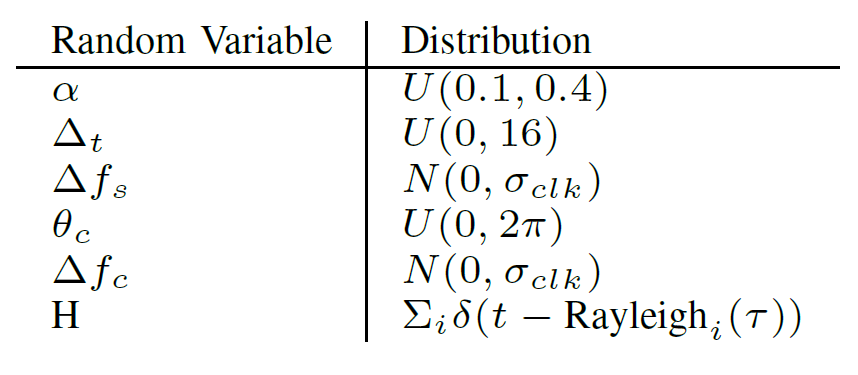
\includegraphics[scale=0.25]{random_variables.png}
	\caption{Random variables used for channel impairments.}
	\end{wrapfigure}
	The synthetic data set consists of several simulated wireless channels. The authors of \cite{ORC} use an audio source, followed by an analog modulator as well as I.I.D. symbol generator followed by a digital modulator. Then the signals are subjected to synthetic channel impairments, all of which with a certain degree of randomness.
	For instance, signal shaping is distributed uniformly as $\alpha \sim U(0.1, 0.4)$, interpolation depends on uniform as well as normal distributions etc. Full model is shown in fig. \ref{sig_gen}.
	
	\begin{figure}\label{sig_gen}
		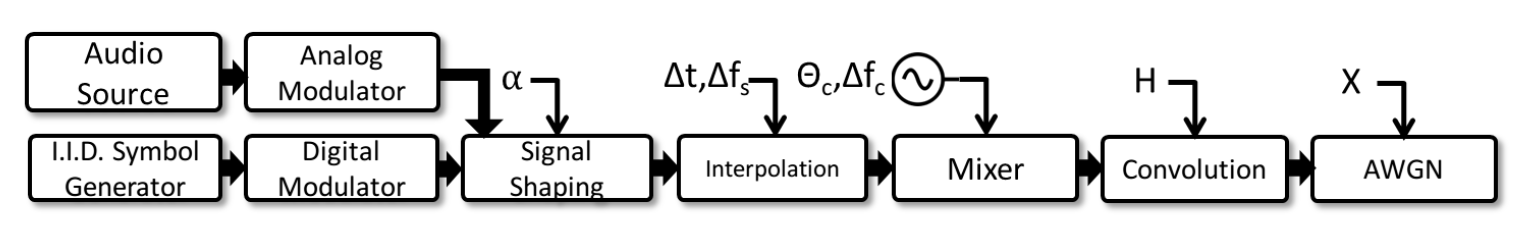
\includegraphics[scale=0.25]{signal_generation.png}
		\caption{Signal generation model in the bechmark dataset.}
	\end{figure}
	
	Furtherly, the synthetic dataset consists of two parts which the authors describe as \textit{normal} classes and \textit{difficult} classes. The normal case consist of 11 signal classes: OOK, 4ASK, BPSK, QPSK, 8PSK, 16QAM, AM-SSB-SC, AM-DSB-SC, FM, GMSK, OQPSK, which are supposedly relatively easy to categorize. The difficult case consists of all 24 classes: OOK, 4ASK, 8ASK, BPSK, QPSK, 8PSK, 16PSK, 32PSK, 16APSK, 32APSK, 64APSK, 128APSK, 16QAM, 32QAM, 64QAM, 128QAM, 256QAM, AM-SSB-WC, AM-SSB-SC, AM-DSB-WC, AM-DSB-SC, FM, GMSK, OQPSK. The simultaneous presence of, for instace,  64APSK and 128APSK, or 128QAM and 256QAM makes these classes much harder to distinguish.
	
	\begin{figure}
	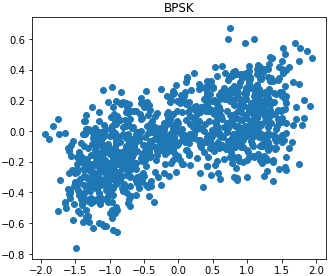
\includegraphics[scale=0.5]{BPSK.png}
	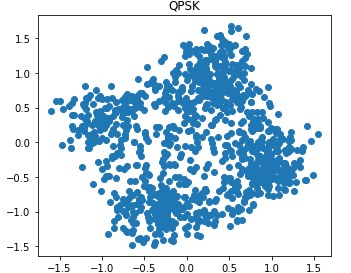
\includegraphics[scale=0.5]{QPSK.png}
	\caption{Examples of signals from the benchmark dataset.}	
	\end{figure}
	
	The authors of \cite{ORC} also provide an OTA part of the dataset in which they transmit and receive signals using a universal software radio peripheral (USRP) B210 software defined radio (SDR). Those signals do not feature any synthetic channel impairments.
		
	For the detailed description of the dataset, see \cite{ORC}, ch. III.
	
	\section{Persistent homology}
	
	\subsection{Basics of homology theory}
	
	\subsection{Topological summaries}
	
	The goal of Topological Data Analysis is to apply homology groups described in the previous section to datasets. The sets in question, however, are in most cases discrete (finite) clouds of points, hence they do not possess topological features such as connectedness or cycles. Therefore the idea is to consider each point along with its neighborhood of a growing radius and monitor the features of the union of such neighborhoods rather than the points themselves (see fig. [...]). For computational purposes, the neighborhoods are then replaced by their simplex counterparts defined below.
	
	\begin{definition}
		Let $A$ be a finite set in a metric space $(X,d)$. The Vietoris-Rips complex of the set $A$ for a fixed $\varepsilon>0$ is the simplicial complex with vertices in $A$ such that the set $\{a_1, \dots, a_n\}\subseteq A$ is a simplex if $d(a_i,a_j)<\varepsilon$ for every $1\leqslant i, j\leqslant n$. We will denote it by $VR_\varepsilon$.
	\end{definition}

As shown in fig. [...], the points in the dataset are surrounded by their respective balls, and then the centers of such balls are connected by a simplex if and only if the distance is sufficiently small. Following this construction we obtain the Vietoris-Rips complex. Obviously, the appearance of simplices is immediately related to the size of $\varepsilon$: the greater $\varepsilon$ becomes, the less strict the criterion is, and the larger number of simplices appear. The crucial method of TDA is observing the topological changes as $\varepsilon$ increases.

\begin{definition}
	A filtration is such a nested family of complexes $(VR_\varepsilon)_{\varepsilon>0}$ that for any $\varepsilon_1, \varepsilon_2>0$ if $\varepsilon_1<\varepsilon_2$ then $VR_{\varepsilon_1} \subseteq VR_{\varepsilon_2}$.
\end{definition}

It is useful to interpret the growing parameter $\varepsilon$ as \textit{time}: as time passes, the complexes in the filtration change and, more precisely, certain topological features appear and disappear or, as is often said in TDA, are born and die. Topological summaries are the means of depiction of the time of birth and death of those features. We will shortly describe a few of the typical summaries.

\subsubsection{Barcodes}

Let $b$ be the time of birth of a feature and let $d$ be the time of its death. A barcode is a representation of the distance $d-b$ in the form of horizontal bars. One can find significant topological features by identifying bars of substantial length. A certain drawback of barcodes is the relative small number of features presented on a single image.

\subsubsection{Persistence diagrams}

Persistence diagrams are summaries which we rely on the most in this paper. Similarly to barcodes, they depict births and deaths of features, however, this time presented in the form of points $(b,d)$ on the plane. Since $b<d$ for every $b,d$, all points of the diagram are stored above the diagonal $d=b$. Formally, a persistence diagram is a multiset, i.e. it allows multiple occurrences of points $(b,d)$, meaning that certain features are born at the same time $b$ and die at the same time $d$.

\subsubsection{Persistence landscapes}

While offering an elegant representation of the lifetimes of features, both the space of barcodes and the space of persistence diagrams lack the structure of a Hilbert space. Persistence landscapes are an attempt to remedy that, transforming a diagram into a sequence of functions. From a practical point of view, a landscape is a 45$^\circ$ clockwise rotation of a persistence diagram. However, a rigorous mathematical definition requires certain care. Our definition follows \cite{BD}. For a birth-death ordered pair $(b,d)$ let $f_{(b,d)}\colon \mathbb{R}\to [0, \infty]$ be the following piecewise linear function:
$$f_{(b,d)}(x) = \begin{cases}
0 \:\: & \text{if } x \notin (b,d) \\
x-b \:\: & \text{if } x\in (b, \frac{b+d}{2}] \\
-x+d \:\: & \text{if } x\in (\frac{b+d}{2},d) .
\end{cases}$$
The persistence landscape is the sequence of functions $\lambda_k \colon \mathbb{R} \to [0,\infty], k\in\{1,2,3,\ldots\}$, such that $\lambda_k(x)$ is the $k$-th largest value of $\{ f_{(b_i,d_i)} (x)\}_{i=1}^n$. Additionally put $\lambda_k(x)=0$ if the $k$-th largest value does not exist.

(...)

\section{Description of the applied methods}

	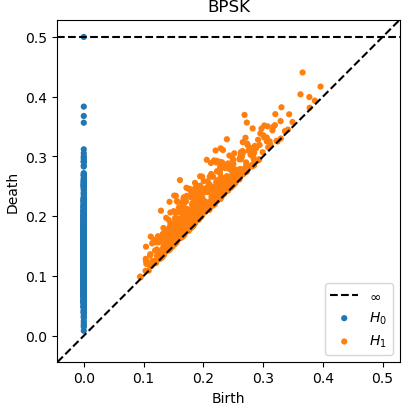
\includegraphics[scale=0.6]{BPSK_diagram.png}	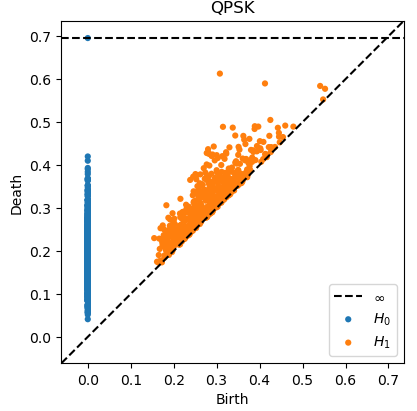
\includegraphics[scale=0.6]{QPSK_diagram.png}
	
\section{Main results}
	
	\begin{thebibliography}{10}
		
		\bibitem{BZCAM}
		R. Borkowski, D. Zibar, A. Caballero, V. Arlunno, I.T. Monroy \emph{Stokes Space-Based Optical Modulation Format Recognition for Digital Coherent Receivers}, IEEE Photonics Technology Letters {\bf 25} (2013), no. 21, 2129-2132.
		
		\bibitem{BD}
		P. Bubenik, P. D�otko \emph{A persistence landscapes toolbox for topological statistics}, 	Journal of Symbolic Computation, {\bf 78} (2017), 91-114.
		
		\bibitem{ChM}
		F. Chazal, B. Michel, \emph{An introduction to Topological Data Analysis: fundamental and practical aspects for data scientists}, Frontiers in Artificial Intelligence \textbf{4} (2021), 1-28.
		
		\bibitem{Dobre}
		O.A. Dobre, A. Abdi, Y. Bar-Ness, W. Su \emph{Survey of Automatic Modulation Classification Techniques: Classical Approaches and New Trends}, IET Communications {\bf 1} (2007), no. 2, 137-156.
		
		\bibitem{ORC}
		T.J. O'Shea, T. Roy, T.C. Clancy \emph{Over the Air Deep Learning Based Radio Signal Classification}, IEEE Journal of Selected Topics in Signal Processing {\bf 12} (2018), no. 1, 168-179.
		
	\end{thebibliography}
	
	
	
\end{document}
